% --- UNIVERSAL PREAMBLE BLOCK ---
\documentclass[aspectratio=169, 11pt]{beamer}
\usepackage{fontspec}
\usepackage[english, bidi=basic, provide=*]{babel}
\babelprovide[import, onchar=ids fonts]{english}

% Set default fonts to Noto Sans
\babelfont{rm}{Noto Sans}
\babelfont{sf}{Noto Sans}

% Required for table/figure adjustments
\usepackage{booktabs}
\usepackage{graphicx}

% --- BEAMER THEME & CUSTOMIZATION ---
\usetheme{Madrid}
\usefonttheme{professionalfonts}

% Customizing colors to match BrainBuzz UI (Green)
\definecolor{BrainBuzzGreen}{RGB}{22, 163, 74} % Tailwind green-600
\setbeamercolor{structure}{fg=BrainBuzzGreen}
\setbeamercolor{palette primary}{bg=BrainBuzzGreen, fg=white}
\setbeamercolor{palette secondary}{bg=BrainBuzzGreen!80!black, fg=white}
\setbeamercolor{palette tertiary}{bg=BrainBuzzGreen!60!black, fg=white}
\setbeamercolor{title}{bg=white, fg=BrainBuzzGreen}
\setbeamercolor{item}{fg=BrainBuzzGreen}

% Remove navigation symbols for a cleaner look
\setbeamertemplate{navigation symbols}{}

% --- TITLE PAGE INFORMATION ---
\title[BrainBuzz: MCQ Platform]{BrainBuzz}
\subtitle{An Automated MCQ-Based Quiz Platform}
\author[]{
    Abhishek Yadav \and Aditya Pal \and Antrikshya Gupta \and \\
    Archit Saxena \and Ayush Sharma
}
\institute[]{
    Branch: CSE-R (B.Tech Sem 4) \\
    Subject Code: ICS-454 (Mini Project)
}
\date{} % Suppresses date from both title slide and bottom footer

% --- DOCUMENT BEGINS ---
\begin{document}

% 1. Title Slide
\begin{frame}
    \titlepage
\end{frame}

% Table of Contents
\begin{frame}{Presentation Outline}
    \tableofcontents[hideallsubsections]
\end{frame}

% 2. Introduction
\section{Introduction}
\begin{frame}{Introduction}
    \textbf{The Shift to Digital Education}
    \begin{itemize}
        \item The education sector is rapidly digitizing, yet many academic assessments remain heavily reliant on manual processes.
        \item \textbf{Traditional Methods:} Paper-based quizzes demand significant manual effort for administration, checking, and result compilation.
        \item \textbf{Online Forms:} Standardized web forms often lack the robust security, strict time controls, and attempt restrictions required for academic integrity.
    \end{itemize}
    \vspace{0.5cm}
    \textbf{The BrainBuzz Solution}
    \begin{itemize}
        \item A dedicated, secure, and automated examination platform tailored for educational institutes to streamline the entire assessment lifecycle.
    \end{itemize}
\end{frame}

% 3. Problem Statement
\section{Problem Statement}
\begin{frame}{Problem Statement}
    Current digital makeshift solutions present critical vulnerabilities and inefficiencies:
    \vspace{0.3cm}
    \begin{itemize}
        \item \textbf{Vulnerability to Academic Dishonesty:} Basic forms fail to enforce strict attempt limits, allowing students to resubmit answers.
        \item \textbf{Predictable Assessments:} A lack of dynamic question randomization makes answer-sharing and cheating trivial.
        \item \textbf{Inefficient Evaluation Process:} Educators spend disproportionate amounts of time manually grading papers and cross-referencing answers.
        \item \textbf{Lack of Actionable Insights:} Existing methods offer no automated, structured way to visualize and analyze cohort performance instantly.
    \end{itemize}
\end{frame}

% 4. Objectives
\section{Objectives}
\begin{frame}{Project Objectives}
    \begin{itemize}
        \item \textbf{Enforce Security \& Integrity:} Deploy a platform that strictly restricts students to a single, authenticated attempt per quiz.
        \item \textbf{Automate Evaluation:} Engineer an instantaneous grading system that automatically evaluates answers and generates definitive scores.
        \item \textbf{Maximize Educator Efficiency:} Create an intuitive interface for rapid quiz creation and frictionless link sharing.
        \item \textbf{Deliver Comprehensive Analytics:} Provide educators with an organized, data-rich dashboard for immediate result interpretation and tracking.
    \end{itemize}
\end{frame}

% 5. Proposed System / Features
\section{Proposed System Features}
\begin{frame}{Proposed System \& Key Features}
    \begin{itemize}
        \item \textbf{Dedicated Teacher Portal:} A secure, authenticated dashboard empowering faculty to design quizzes, manage questions, and visualize results.
        \item \textbf{Frictionless Student Access:} Hassle-free entry via shareable links. Students authenticate using only their Roll Number to begin—eliminating sign-up friction.
        \item \textbf{Dynamic Fair Assessment:} The system enforces rigorous academic standards by randomizing question delivery and strictly barring duplicate attempts.
        \item \textbf{Instant Auto-Evaluation:} Real-time score calculation engine that evaluates submissions and commits data to persistent storage immediately.
    \end{itemize}
\end{frame}

% 6. System Architecture
\section{System Architecture}
\begin{frame}{System Architecture}
    Our application utilizes a modern, decoupled 3-tier architecture:
    \vspace{0.3cm}
    \begin{itemize}
        \item \textbf{Client Tier (Frontend):} 
        \begin{itemize}
            \item Built with \textbf{React.js}.
            \item Delivers a highly responsive, stateful user interface for both the Teacher Dashboard and the Student Quiz Execution window.
        \end{itemize}
        \item \textbf{Application Tier (Backend):} 
        \begin{itemize}
            \item Powered by \textbf{Node.js \& Express.js}.
            \item Handles RESTful API requests, enforces session validation, and processes core quiz evaluation logic.
        \end{itemize}
        \item \textbf{Data Tier (Database):} 
        \begin{itemize}
            \item Hosted on \textbf{MongoDB Atlas}.
            \item Provides scalable, secure NoSQL document storage for student profiles, quiz schemas, and submission analytics.
        \end{itemize}
    \end{itemize}
\end{frame}

% 7. Tools & Technologies
\section{Tools \& Technologies}
\begin{frame}{Tools \& Technologies Utilized}
    Developed completely using the \textbf{MERN Stack}:
    \vspace{0.3cm}
    \begin{itemize}
        \item \textbf{Frontend:} React.js, HTML5, Tailwind CSS (for rapid, modern styling), Lucide React (for iconography).
        \item \textbf{Backend:} Node.js runtime, Express.js framework.
        \item \textbf{Database:} MongoDB Atlas (Cloud Database).
        \item \textbf{Core Language:} JavaScript (ES6+).
        \item \textbf{Security \& Authentication:} 
        \begin{itemize}
            \item \textbf{JWT (JSON Web Tokens):} For stateless, secure API authorization.
            \item \textbf{Bcrypt:} For cryptographic hashing of user passwords.
        \end{itemize}
    \end{itemize}
\end{frame}

% 8. Implementation Details
\section{Implementation Details}
\begin{frame}{Technical Implementation}
    \begin{itemize}
        \item \textbf{Teacher Dashboard Routing:} Implemented protected React routes requiring valid JWTs, allowing faculty to configure metadata (time limits) and inject questions into the database.
        \item \textbf{Quiz Interface State Management:} Designed a distraction-free, locked-down UI that dynamically fetches the question array, tracks current selections in React state, and manages countdown timers.
        \item \textbf{Result Processing Engine:} Upon final submission, the backend securely compares the payload against the encrypted answer key, computes the final integer score, and atomically updates the MongoDB results collection.
    \end{itemize}
\end{frame}

% 9. Working / Screenshots
\section{Working of the System}

% Screenshot 1
\begin{frame}{Working of the System: Landing Page}
    \centering
    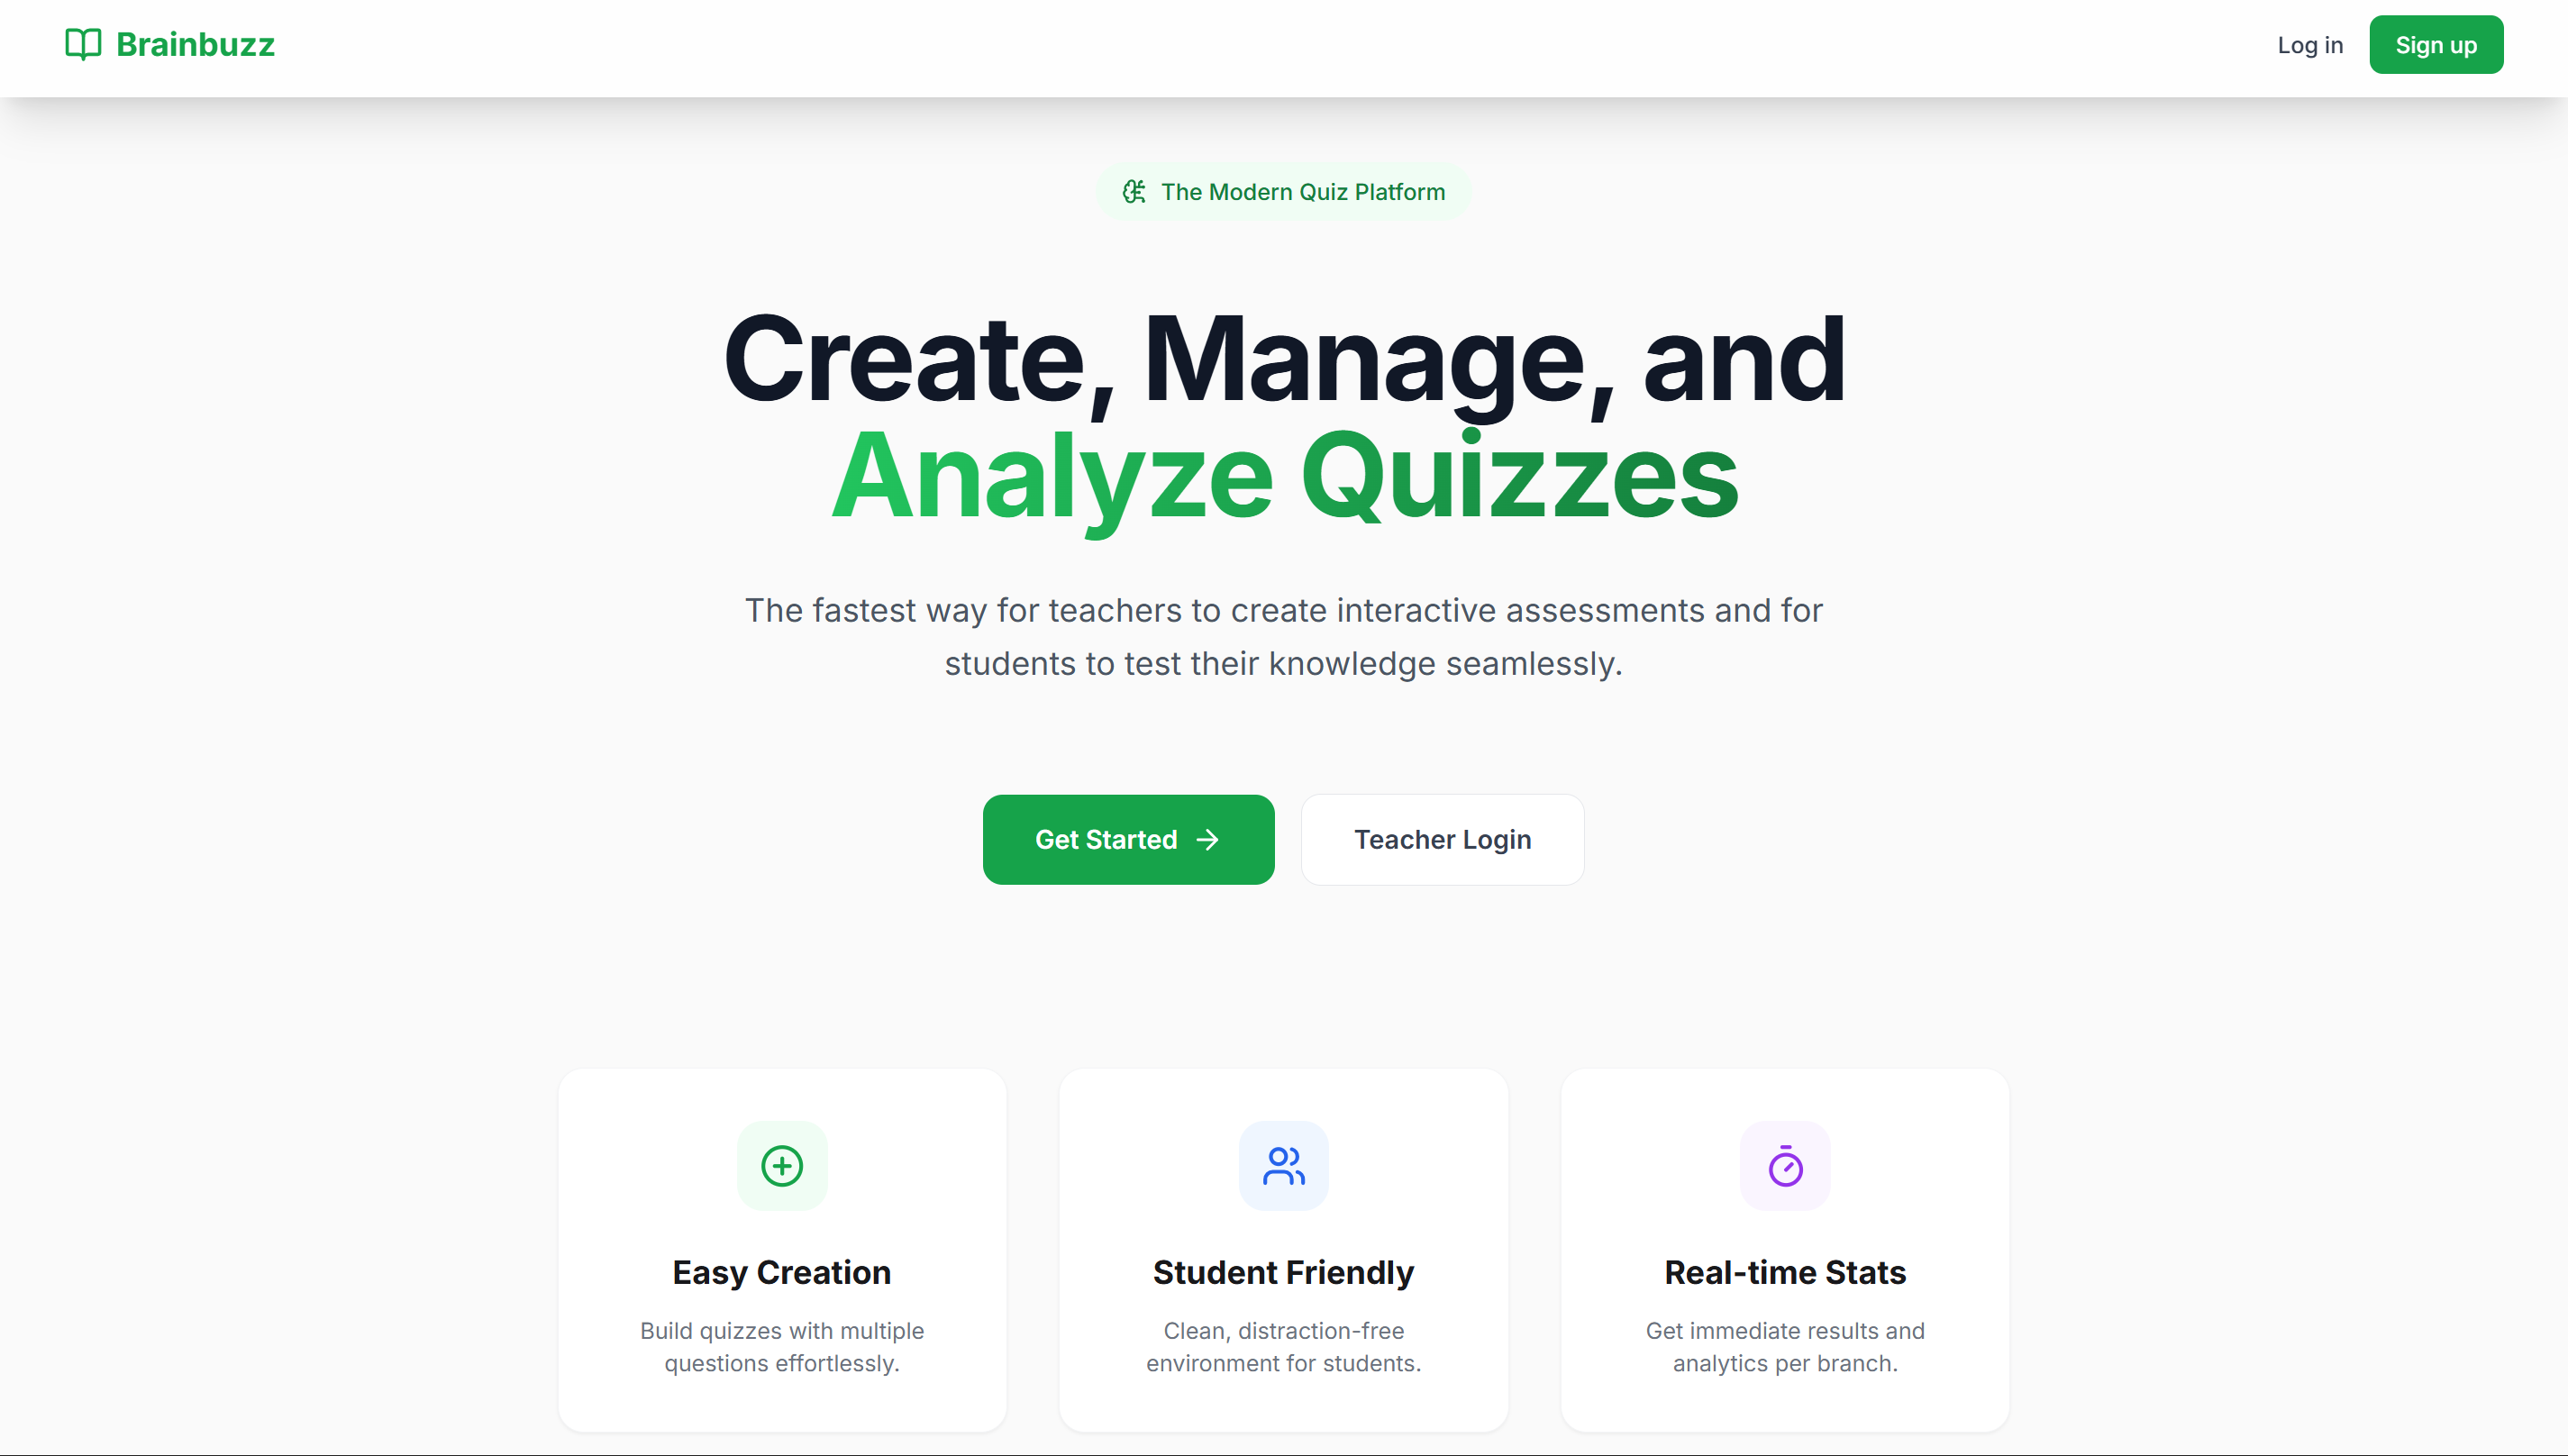
\includegraphics[width=0.85\textwidth]{landing.png}
\end{frame}

% Screenshot 2
\begin{frame}{Working of the System: Authentication}
    \centering
    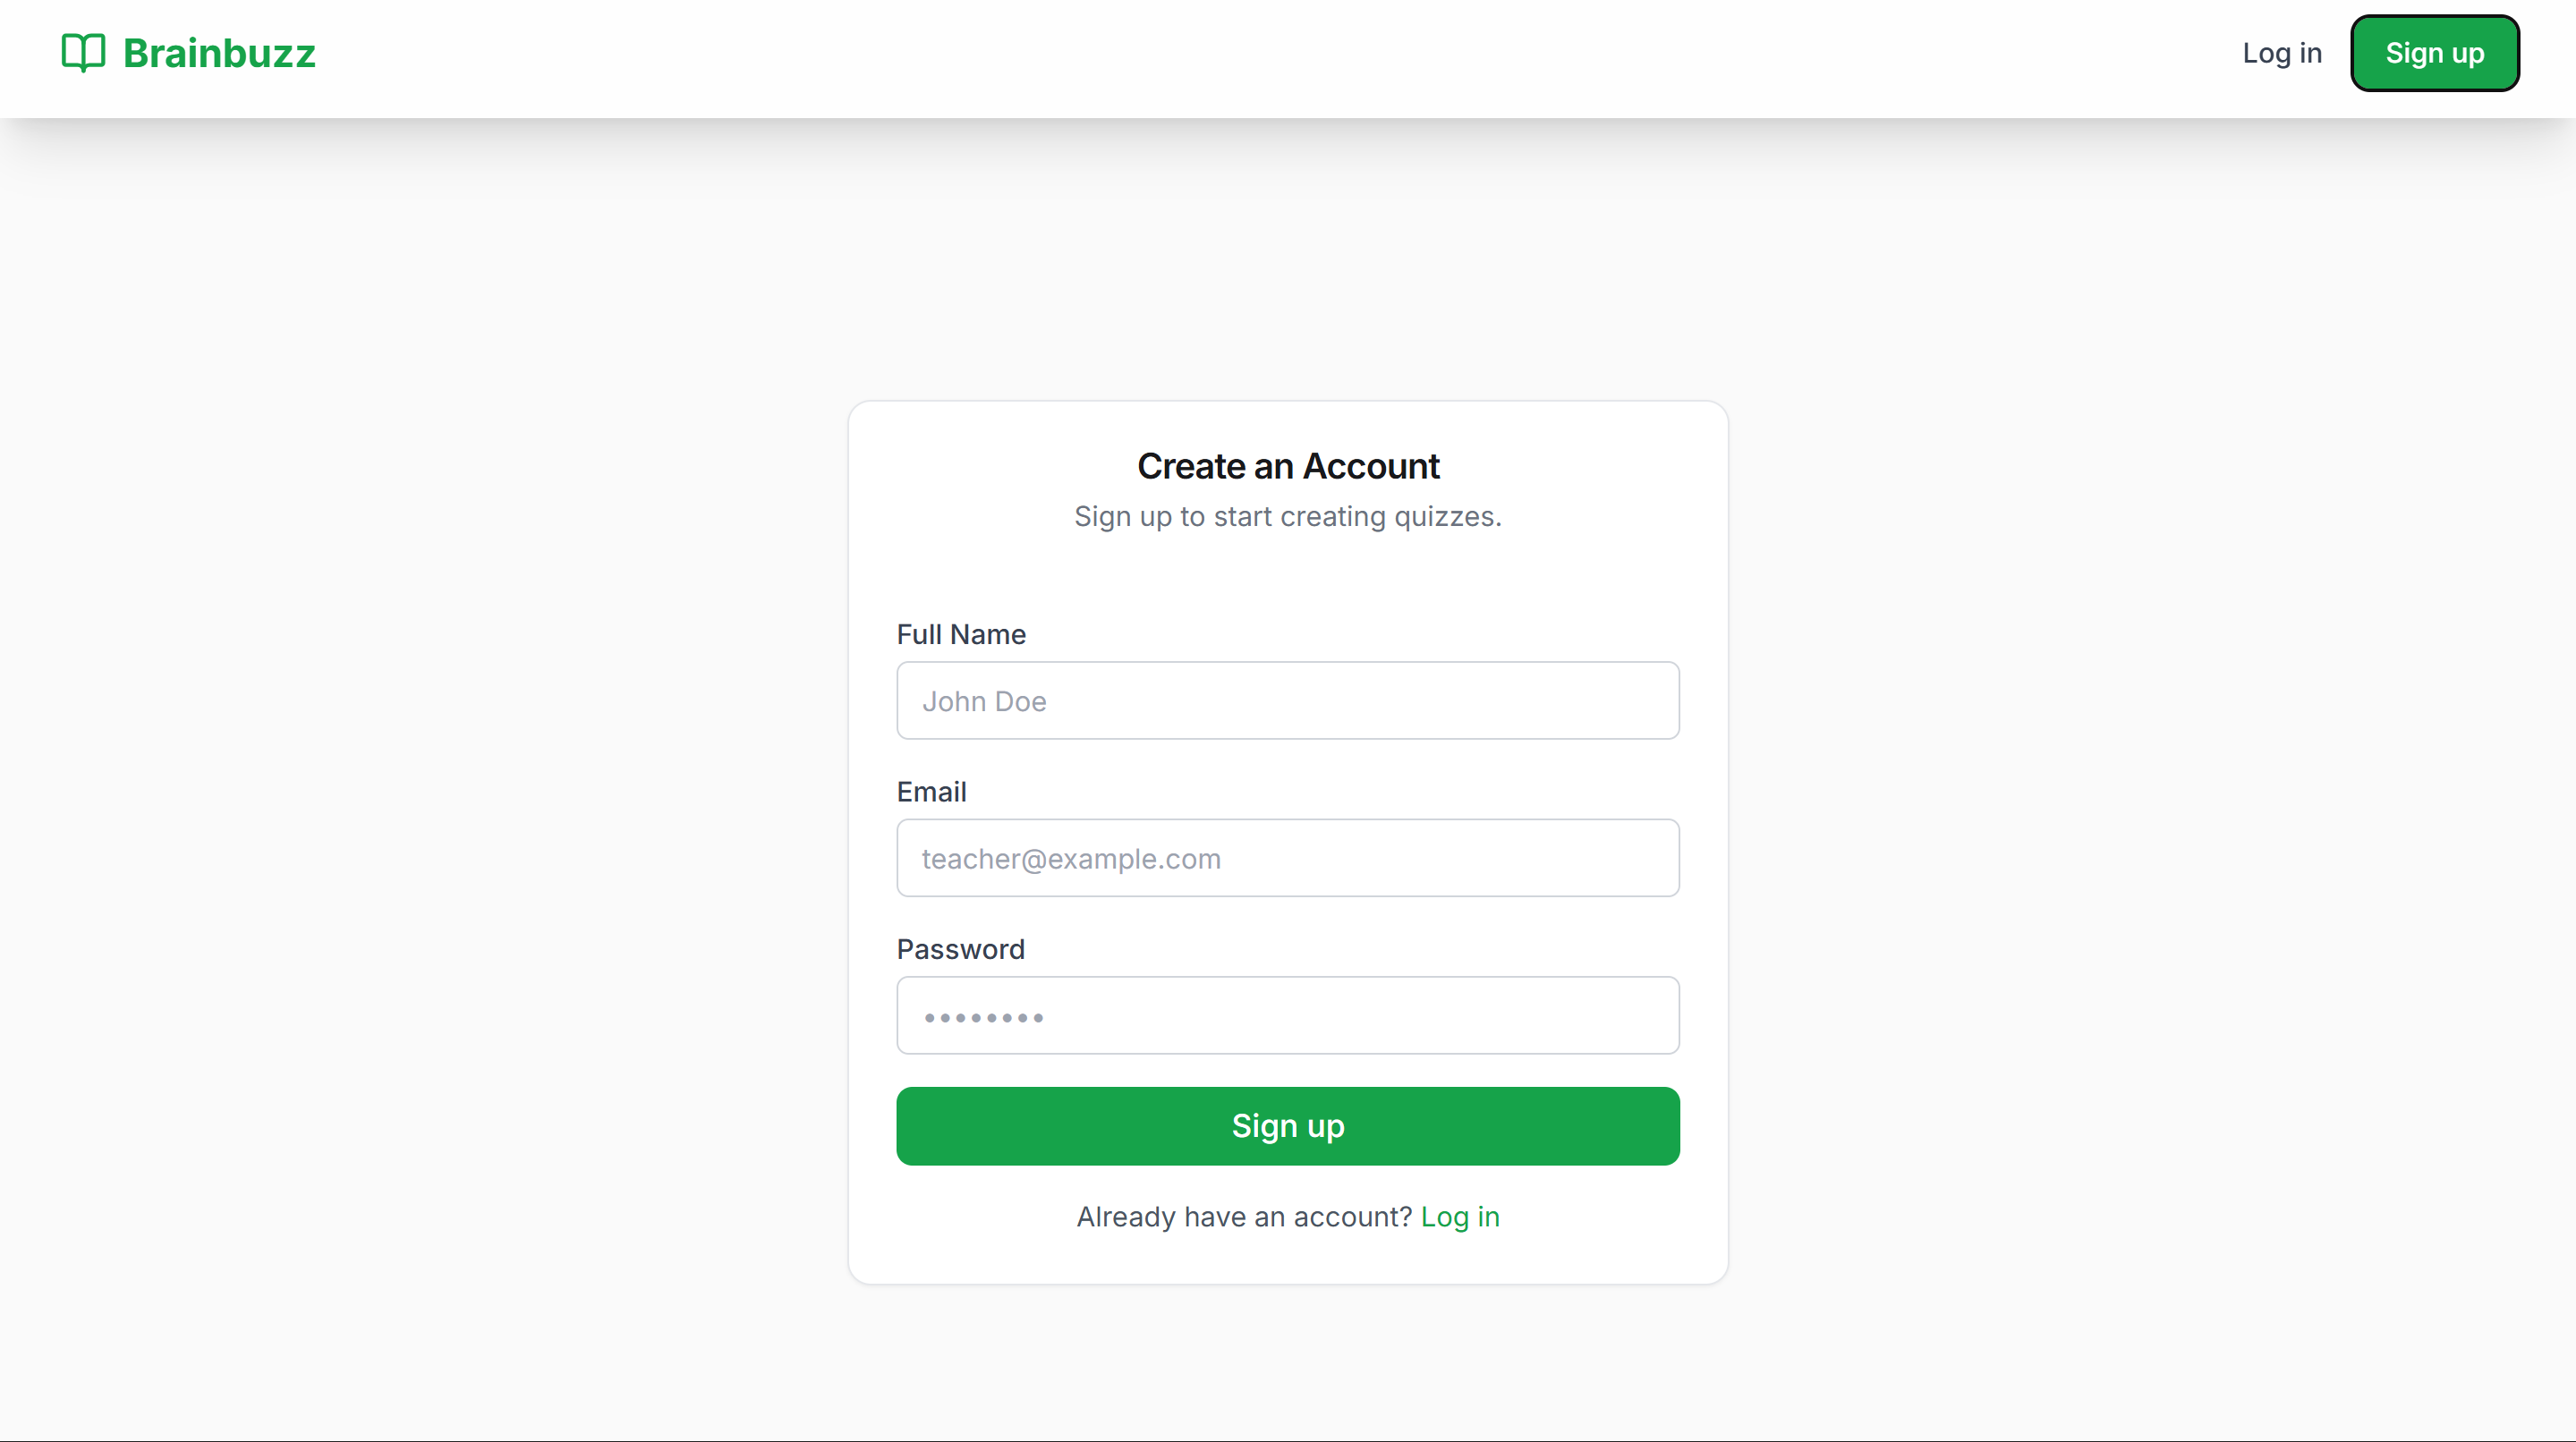
\includegraphics[width=0.85\textwidth]{login.png}
\end{frame}

% Screenshot 3
\begin{frame}{Working of the System: Quiz Creation}
    \centering
    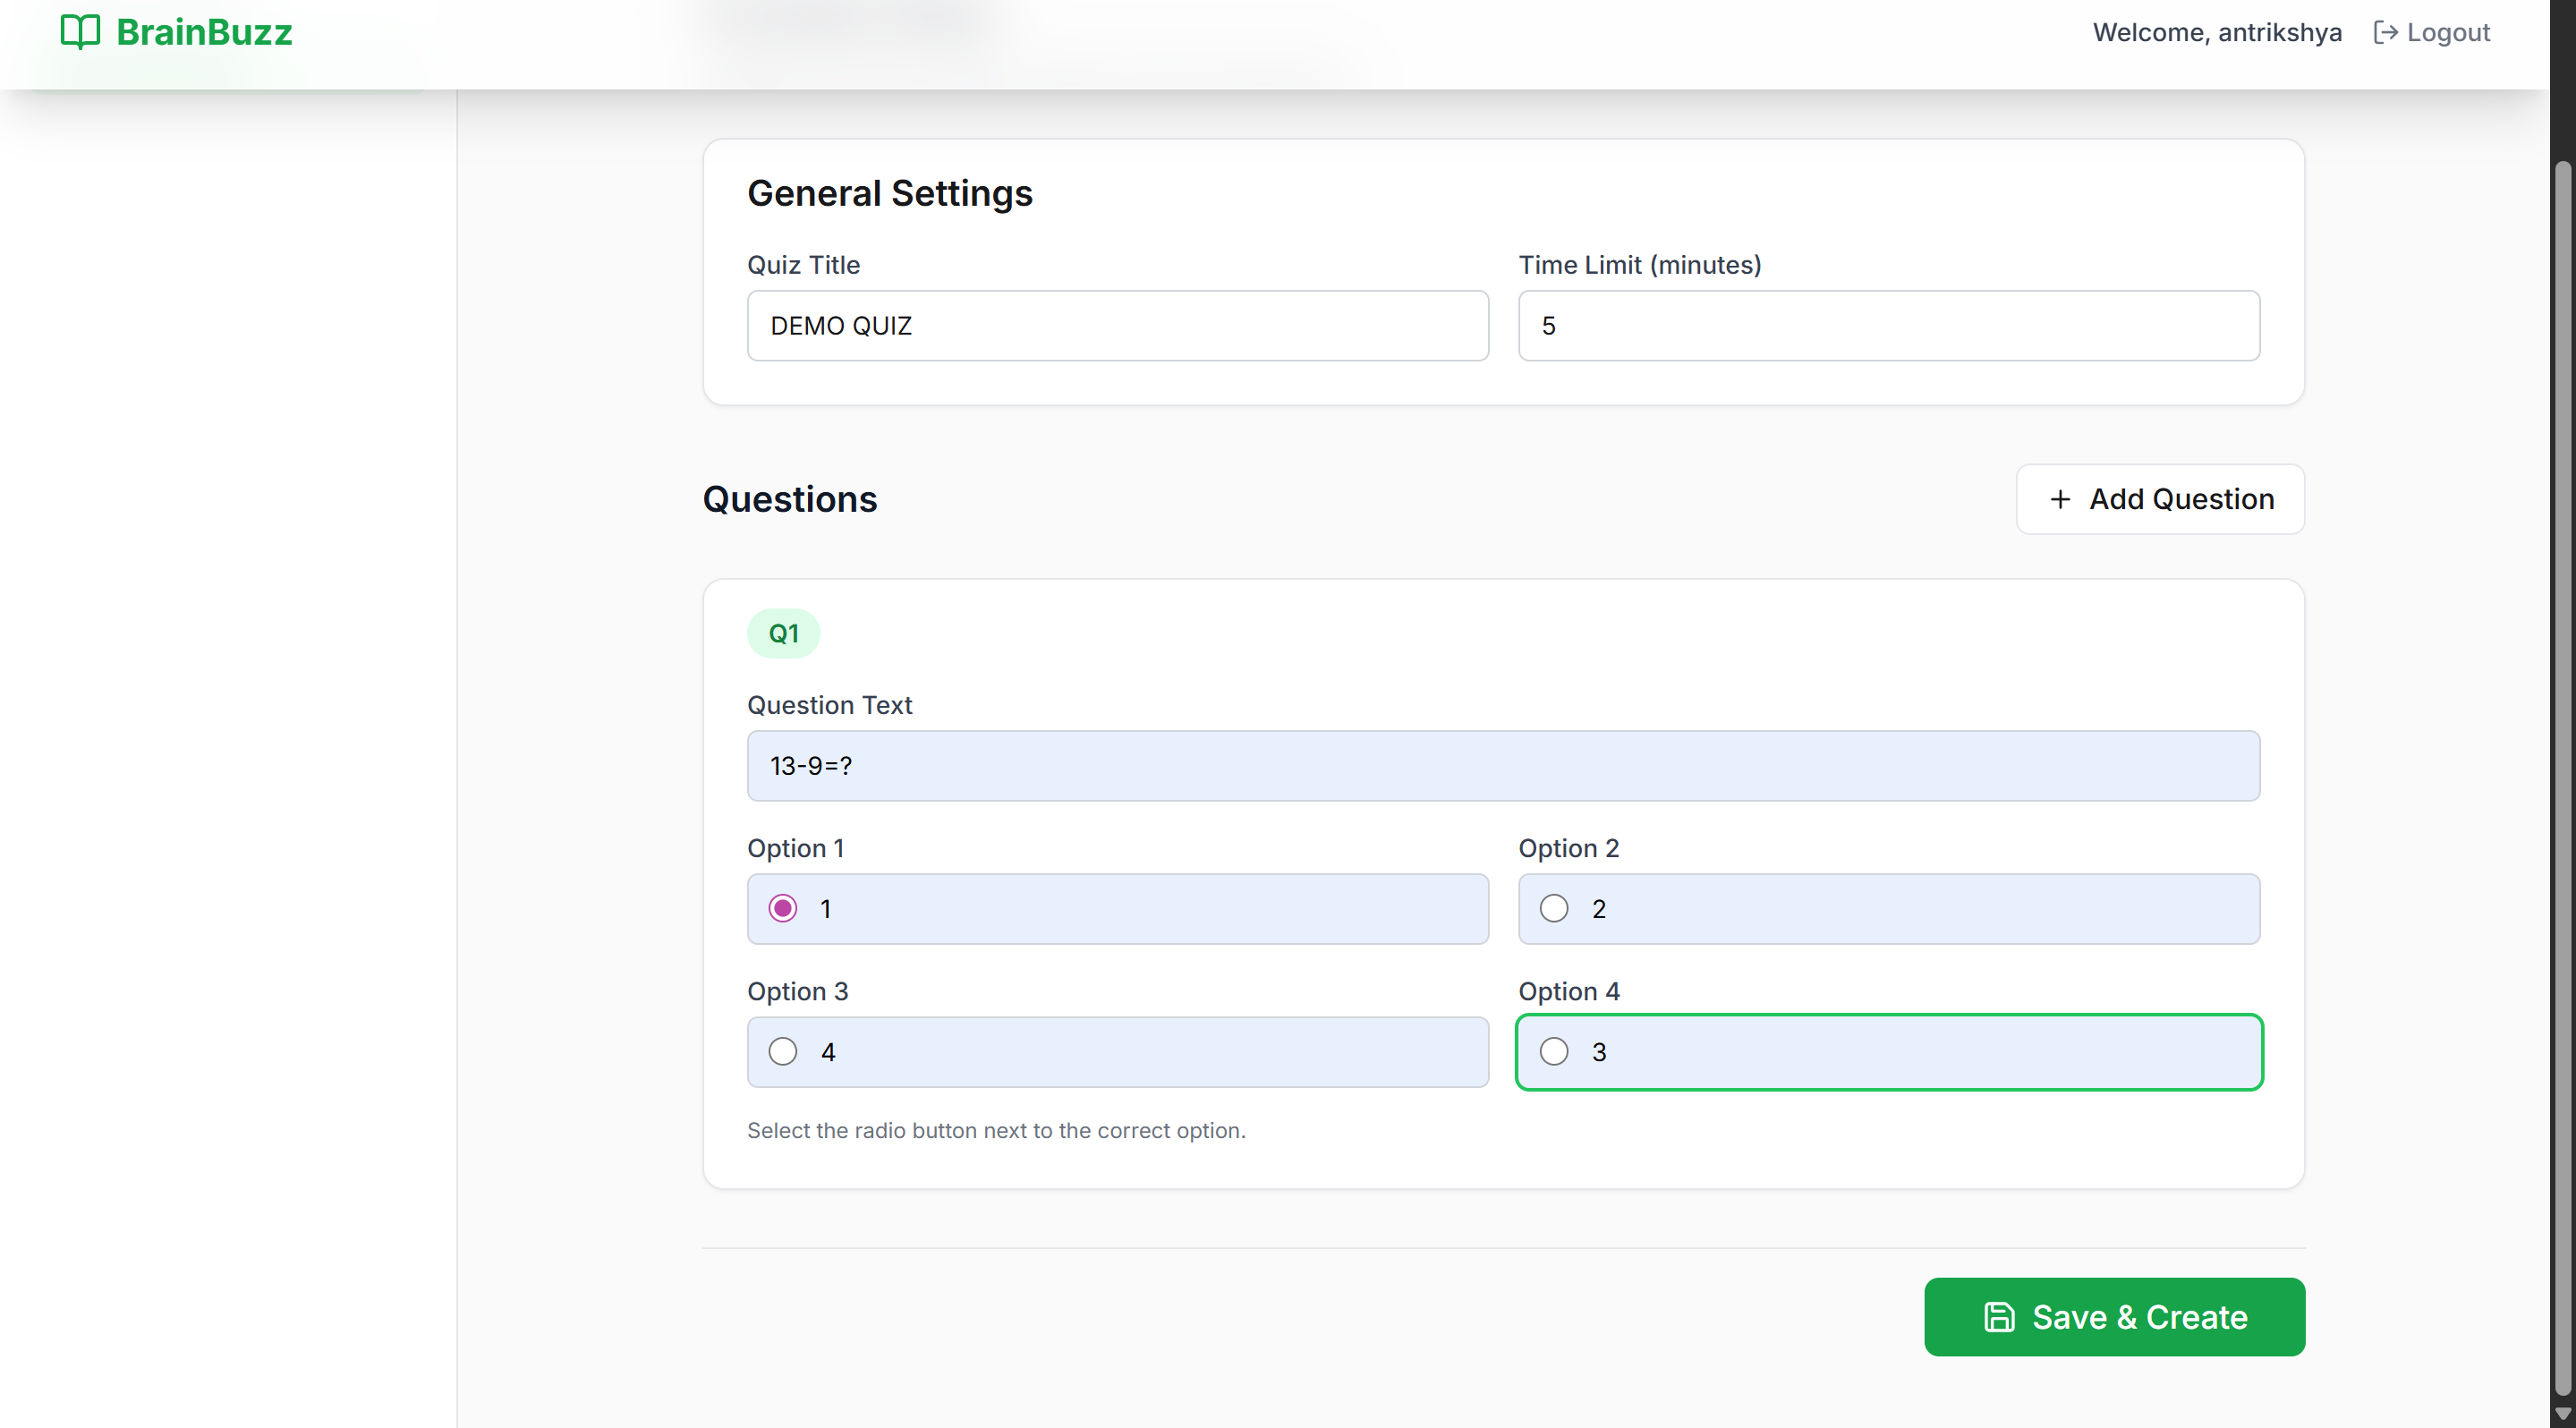
\includegraphics[width=0.85\textwidth]{quiz.png}
\end{frame}

% Screenshot 4
\begin{frame}{Working of the System: Teacher Dashboard}
    \centering
    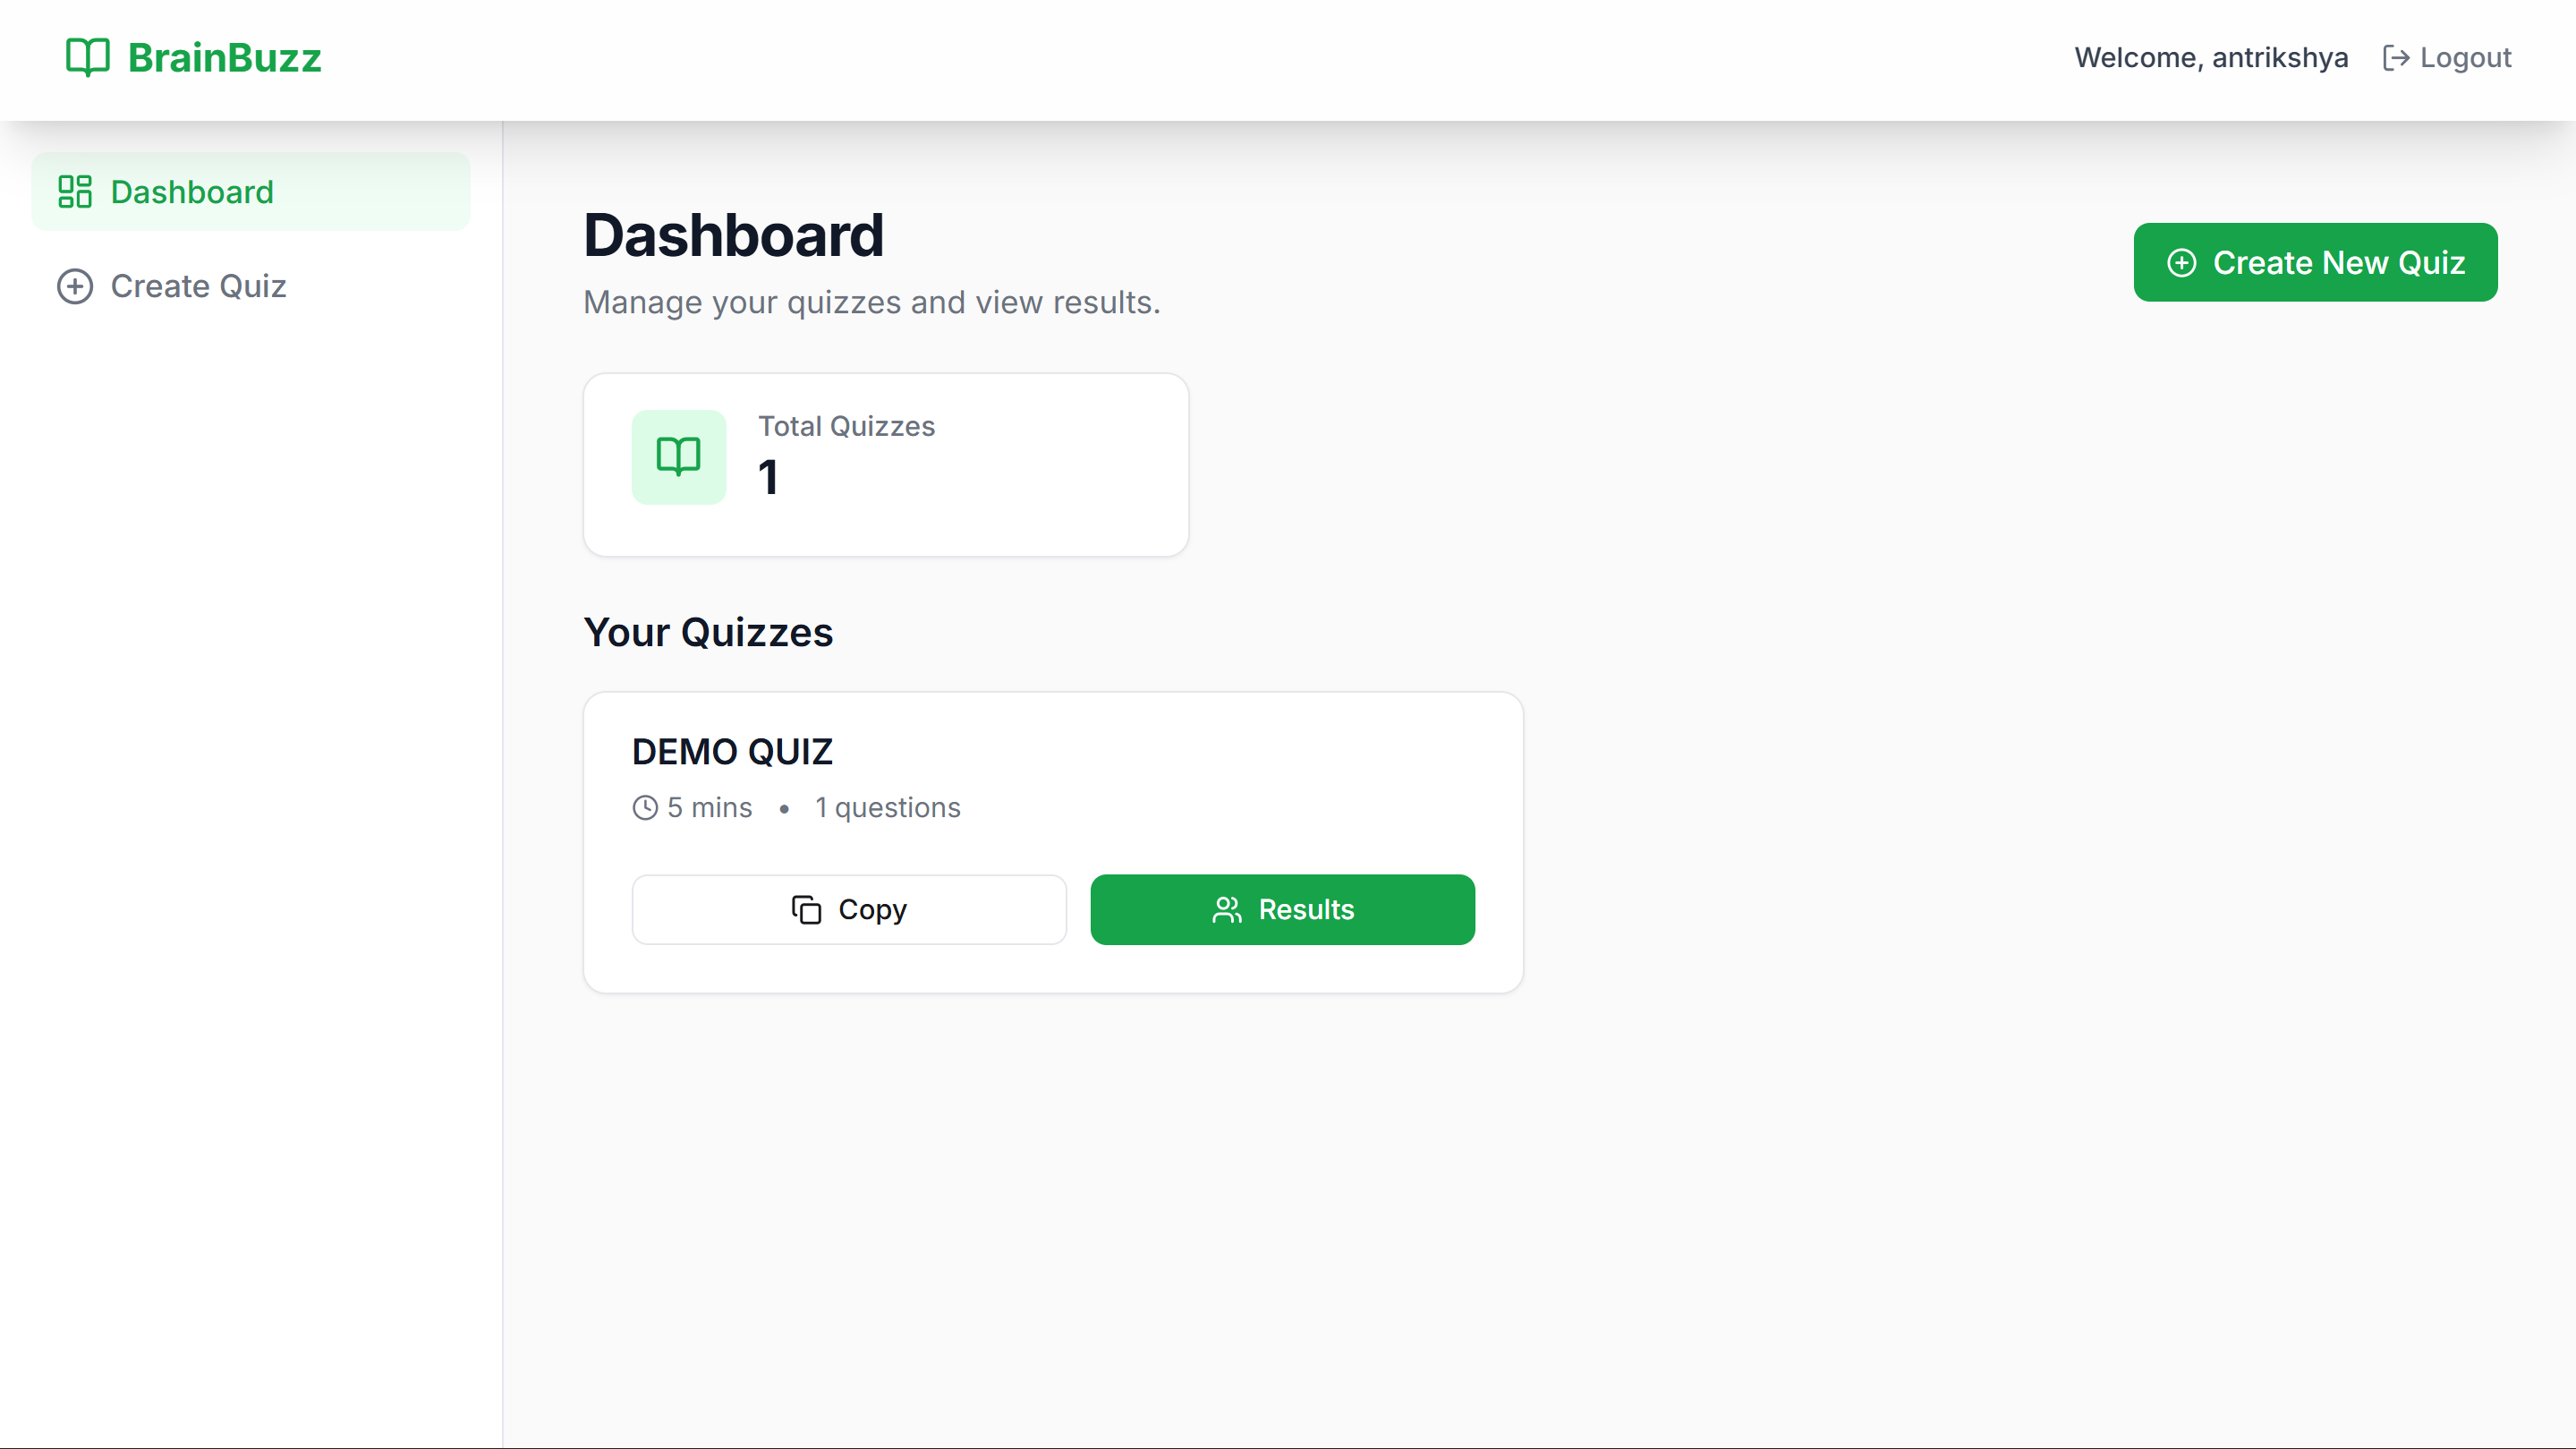
\includegraphics[width=0.85\textwidth]{dashboard.png}
\end{frame}

% Screenshot 5
\begin{frame}{Working of the System: Automated Analytics}
    \centering
    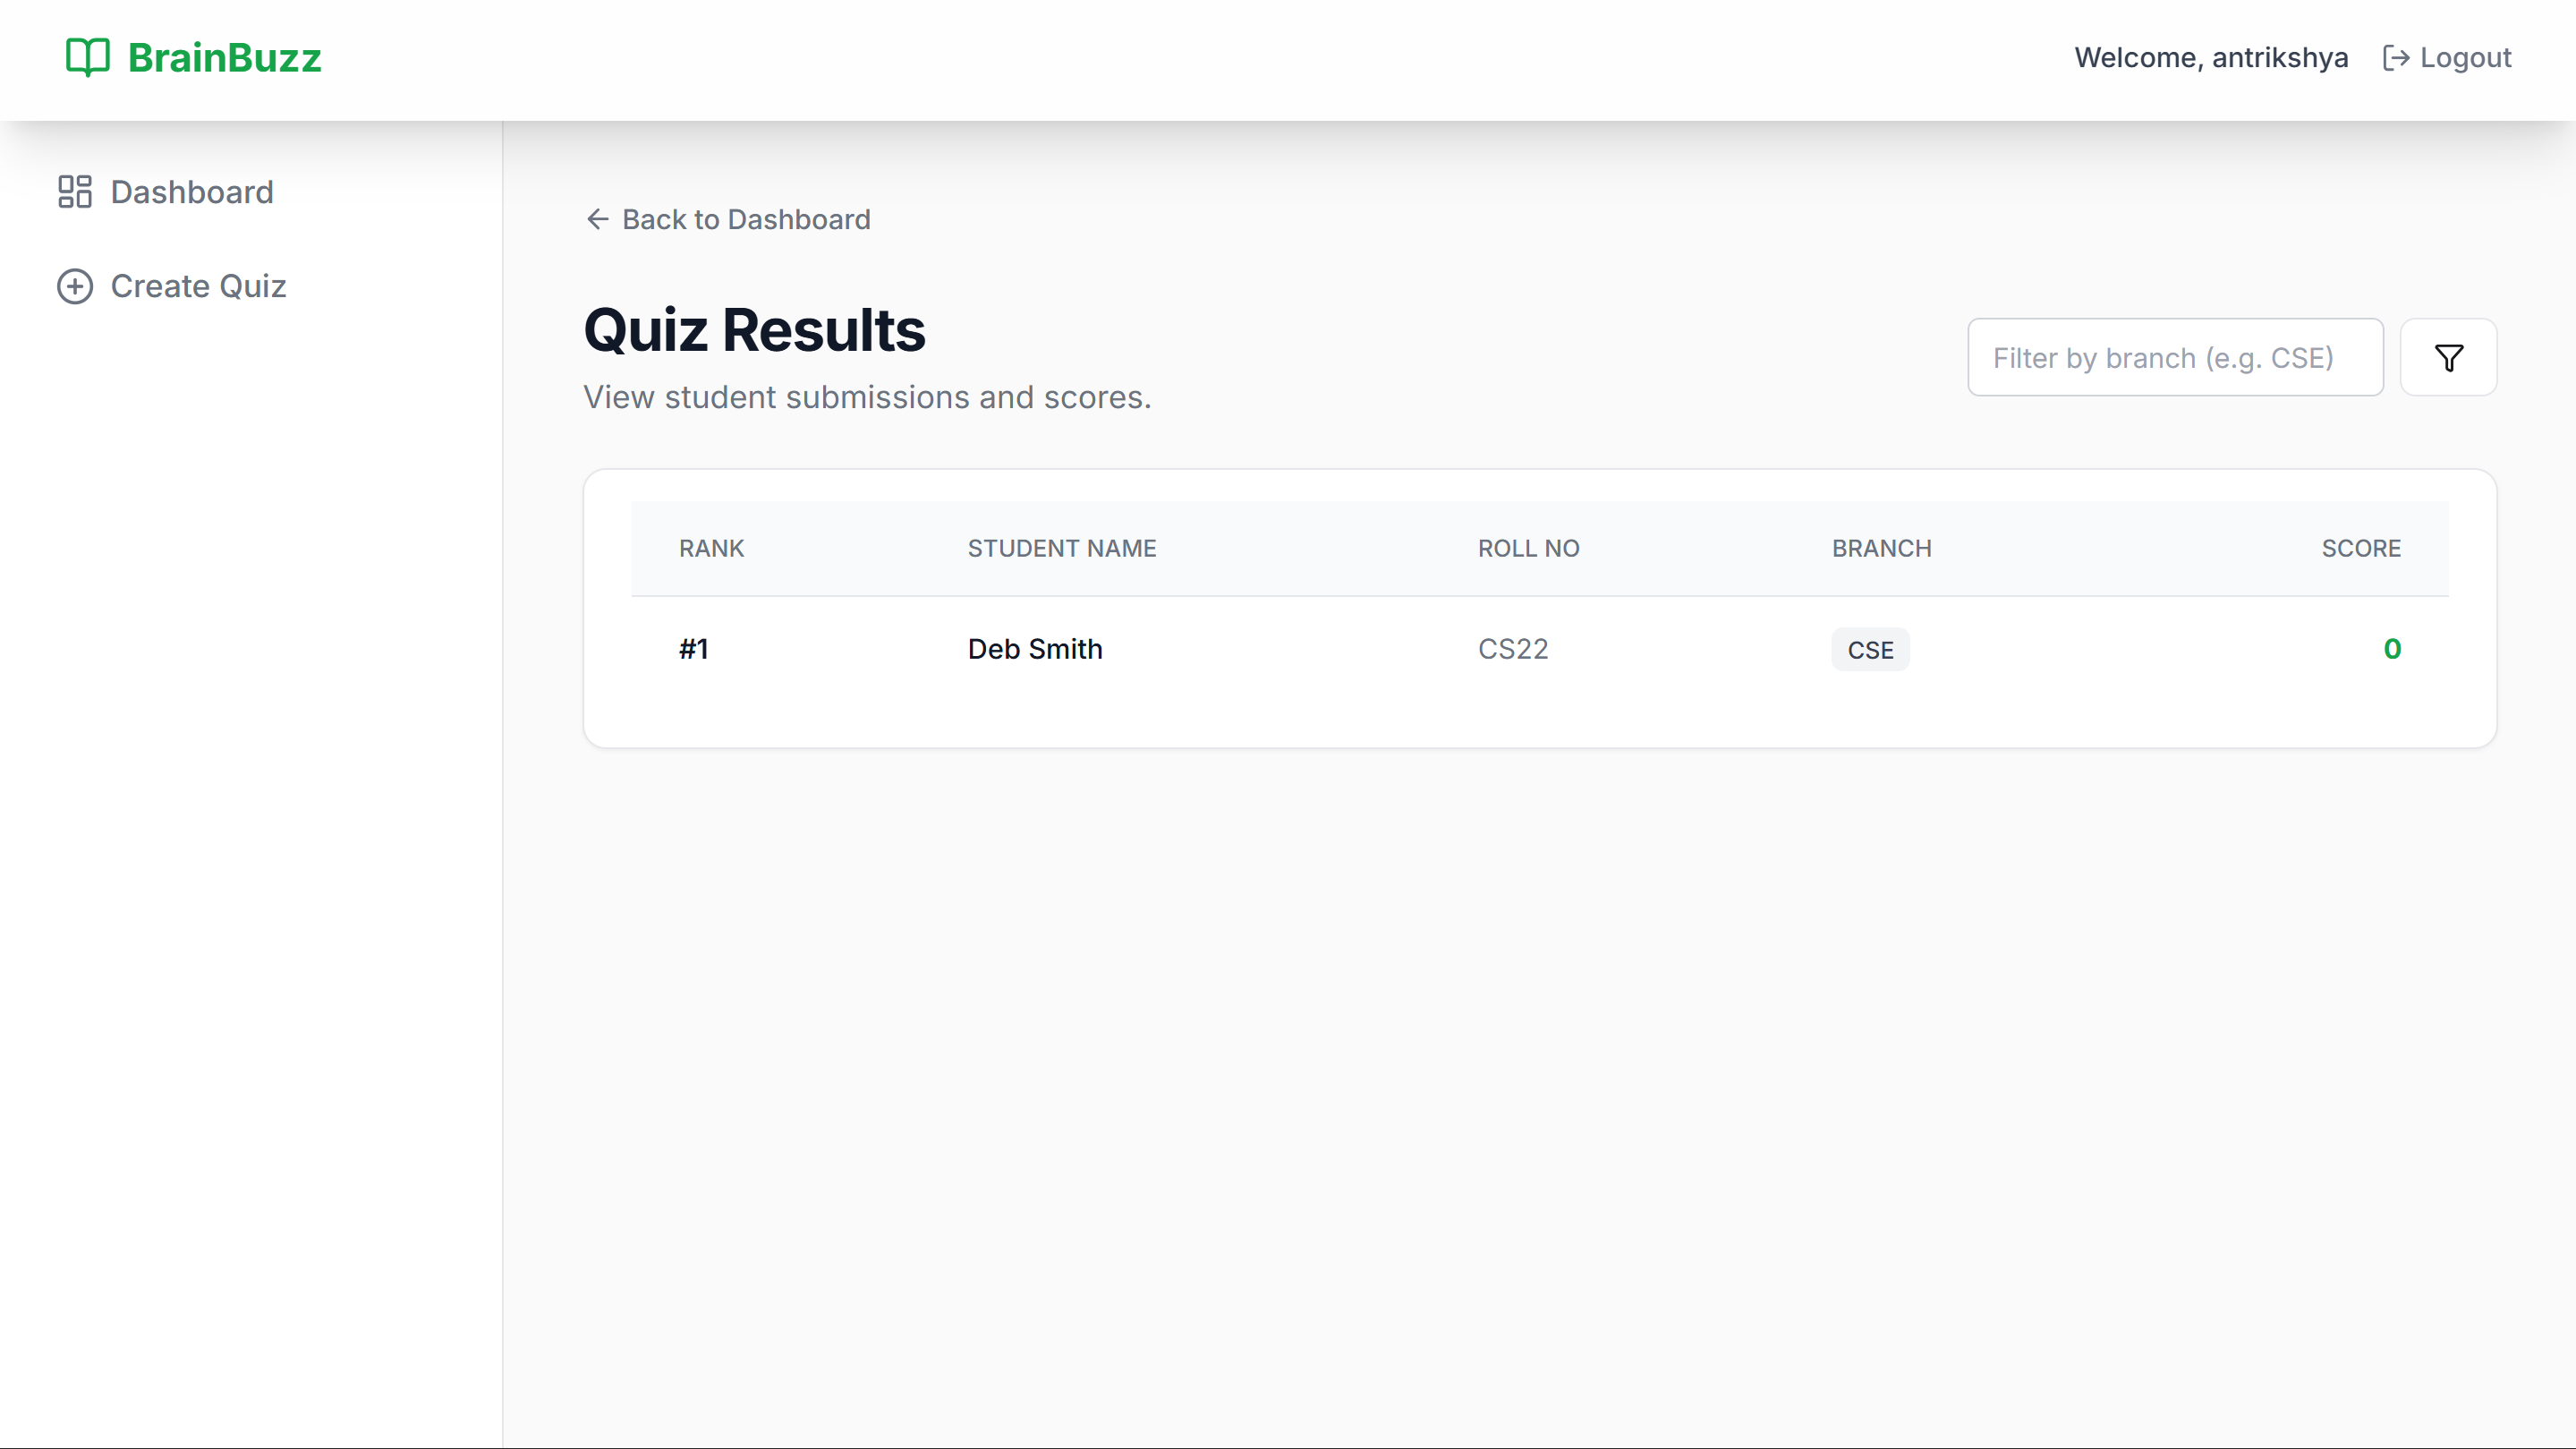
\includegraphics[width=0.85\textwidth]{results.png}
\end{frame}


% 10. Results
\section{Results}
\begin{frame}{Project Results \& Efficacy}
    \begin{itemize}
        \item \textbf{Operational Success:} The platform was successfully deployed, enabling frictionless registration and seamless quiz generation.
        \item \textbf{Guaranteed Integrity:} The attempt control mechanism effectively neutralized duplicate submissions, ensuring a strict 1-to-1 ratio of students to quiz attempts.
        \item \textbf{Evaluation Accuracy:} Achieved \textbf{100\% mathematical accuracy} in MCQ evaluation, completely eliminating manual grading errors and bias.
        \item \textbf{Data Accessibility:} Results are automatically structured and displayed in a sortable, organized format, reducing faculty data processing time from hours to seconds.
    \end{itemize}
\end{frame}

% 11. Conclusion
\section{Conclusion}
\begin{frame}{Conclusion}
    \begin{block}{Impact Statement}
        "BrainBuzz effectively transforms the traditional, labor-intensive assessment process into a highly secure, efficient, and fully digital workflow."
    \end{block}
    \vspace{0.3cm}
    \textbf{Summary of Impact:}
    \begin{itemize}
        \item Establishes an uncompromised, secure online examination environment.
        \item Drastically reduces administrative and grading overhead for academic faculty.
        \item Promotes absolute fairness through algorithmic randomization and attempt policing.
        \item Empowers institutions with immediate, data-driven insights into student performance.
    \end{itemize}
\end{frame}

% 12. Future Scope
\section{Future Scope}
\begin{frame}{Future Scope}
    \begin{itemize}
        \item \textbf{Persistent Student Profiles:} Implement full student login systems to track longitudinal academic history and progress.
        \item \textbf{Gamification Engine:} Introduce real-time leaderboards to encourage healthy competition and engagement.
        \item \textbf{Advanced Data Export:} Develop one-click compilation tools to download result matrices as Excel/CSV or PDF reports.
        \item \textbf{Cross-Platform Ecosystem:} Expand accessibility by developing dedicated Android and iOS native mobile applications.
        \item \textbf{Global Question Bank:} Create a shared repository allowing faculty to store, tag, and reuse questions across multiple semesters.
    \end{itemize}
\end{frame}

% 13. References
\section{References}
\begin{frame}{References}
    \begin{itemize}
        \item \textbf{React Official Documentation:} \textit{https://react.dev}
        \item \textbf{Node.js Official Documentation:} \textit{https://nodejs.org/docs}
        \item \textbf{MongoDB Manual \& Documentation:} \textit{https://www.mongodb.com/docs}
        \item \textbf{Express.js API Reference:} \textit{https://expressjs.com}
        \item \textbf{MDN Web Docs (Mozilla):} \textit{https://developer.mozilla.org}
    \end{itemize}
\end{frame}

% 14. Thank You
\begin{frame}
    \centering
    \Huge \textbf{Thank You!} \\
    \vspace{1cm}
    \large \textit{Any Questions?}
\end{frame}

\end{document}